\begin{figure}[H]
	\begin{subfigure}{.5\textwidth}\centering
		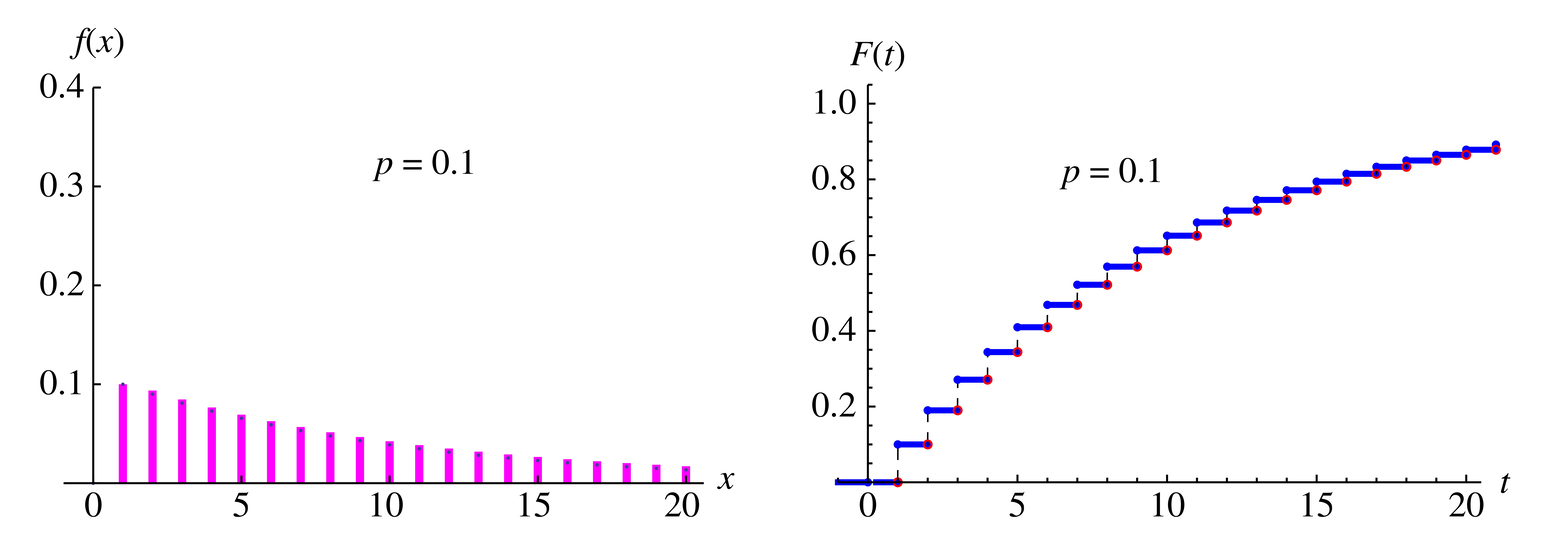
\includegraphics[width=.95\linewidth]{geom.png}
		\caption{Geométrica}
	\end{subfigure}\begin{subfigure}{.5\textwidth}\centering
		\includegraphics[width=.95\linewidth]{binominal.png}
		\caption{Binominal}
	\end{subfigure}
	
	\begin{subfigure}{.5\textwidth}\centering
		\includegraphics[width=.95\linewidth]{negativabinominal.png}
		\caption{Negativa binominal}
	\end{subfigure}\begin{subfigure}{.5\textwidth}\centering
		\includegraphics[width=.95\linewidth]{hyperg.png}
		\caption{Hipergeométrica}
	\end{subfigure}
	
	\begin{subfigure}{.5\textwidth}\centering
		\includegraphics[width=.95\linewidth]{gama.png}
		\caption{$\Gamma$}
	\end{subfigure}\begin{subfigure}{.5\textwidth}\centering
		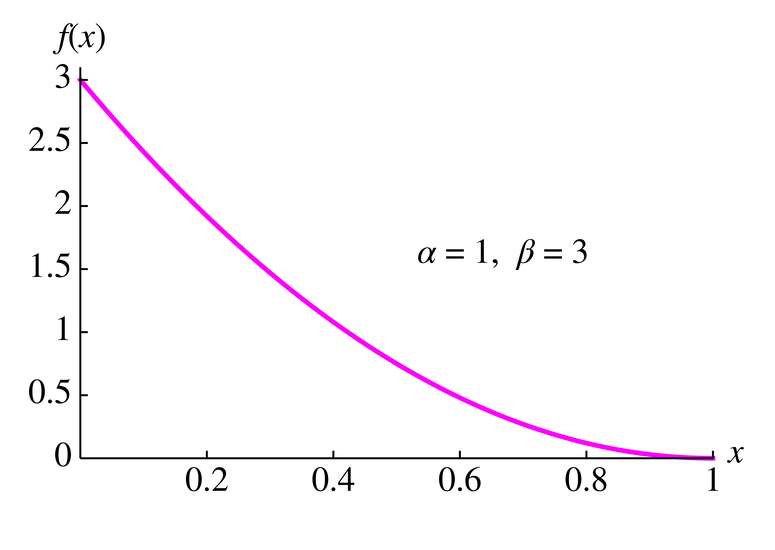
\includegraphics[width=.95\linewidth]{beta.png}
		\caption{Beta}
	\end{subfigure}
	
	\begin{subfigure}{.5\textwidth}\centering
		\includegraphics[width=.95\linewidth]{epsilon_lambda.png}
		\caption{$\epsilon(\lambda)$}
	\end{subfigure}\begin{subfigure}{.5\textwidth}\centering
		\includegraphics[width=.95\linewidth]{normal.png}
		\caption{Normal}
	\end{subfigure}
	
	\begin{subfigure}{.5\textwidth}\centering
		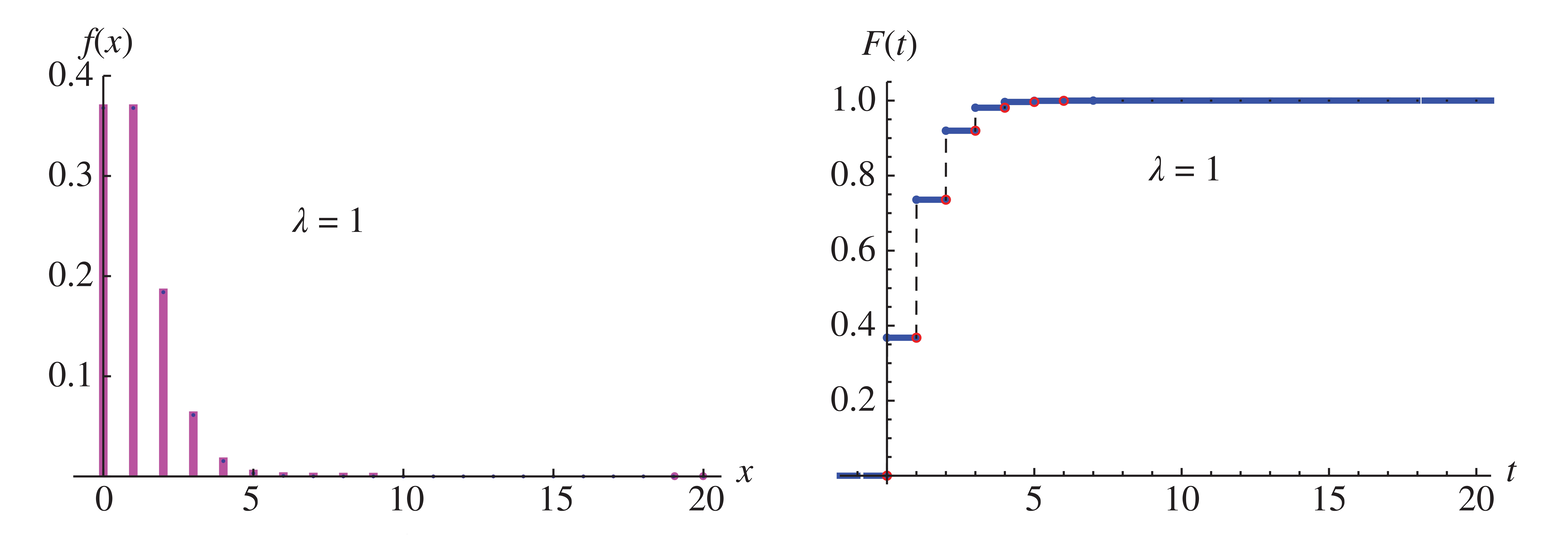
\includegraphics[width=.95\linewidth]{poisson.png}
		\caption{Poisson}
	\end{subfigure}\begin{subfigure}{.5\textwidth}\centering
		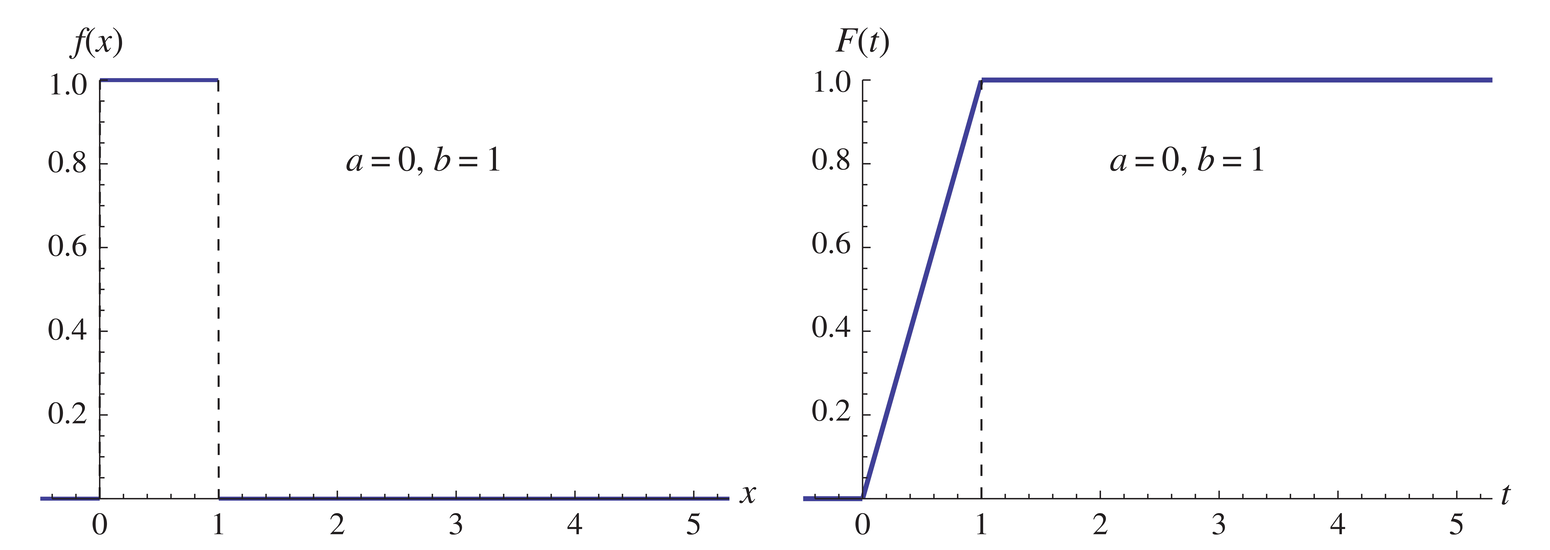
\includegraphics[width=.95\linewidth]{uniforme.png}
		\caption{Uniforme}
	\end{subfigure}
\end{figure}

Una \emph{variable aleatoria} es una función asignando un número real $\mathbb{R}$ a cada posible resultado de un experimento. Con una muestra en espacio $S$, una variable aleatoria $X$ asigna el valor numérico $X(s)$ a cada resultado posible $s$ del experimento. La aleatoriedad viene del hecho que tenemos un experimento aleatorio (con probabilidades descritas por la función de probabilidad $P$). Las variables aleatorias simplifican la notación y expanden la habilidad de cuantificar y resumir resultados de experimentos.

Se dice que una variable $X$ es discreta cuando si hay una lista finita de valores $a_,a_2,\ldots,a_n$ o un una lista infinita de valores $a_,a_2,\ldots$ de tal forma que $P(X=a_j$ para algún $j)=1$. Si $X$ es una variable aleatoria discreta, entonces el conjunto infinito o contable de valores $x$ tal que $P(X=x)$ se llama \emph{soporte} de $X$. En contraste una variable aleatoria continua puede tomar cualquier valor real en un intervalo.
\subsubsection {Función de probabilidad}
La forma más natural de expresar la distribución de variables aleatorias discretas es la \emph{función de probabilidad}\cite{blitz19}*\notad{PMF, por sus siglas en inglés?} que, para una $X$ discreta, es la función $p_X$ dada por $p_X(x)=P(X=x)$. El teorema de \emph{funciones de probabilidad válidas} dice que cuando $X$ es una variable aleatoria con soporte $x1,x2,\ldots$, la función de probabilidad $p_X$ de $x$ debe satisfacer los siguiente criterios:
\begin{itemize}
    \item No negativo $p_X (x) > 0$ si $x=x_j$ para un $j$, y $p_X(x)=0$, de otra forma;
    \item Suma 1: $\sum_{j=1}^{\infty}p_X(x_j)=1$.
\end{itemize}
el primer criterio es verdadero porque la probabilidad es no negativa, el segundo es verdadero ya que $X$ debe tomar \emph{algún} valor, y los eventos ${X=xj}$ están disjuntos, entonces
\begin{equation}
\sum_{j=1}^{\infty}P(X=x_j)=P\bigg(\bigcup_{j=1}^{\infty}\{X=x_j\}\bigg)=P(X=x_1\ \text{ó}\ X=x_2\ \text{ó}\ \ldots)=1.
\end{equation}
\subsubsection {Distribución de Bernoulli y binominal}
Una variable aleatoria tiene la \emph{distribución de Bernoulli} con un parámetro $p$ si $P(X=1)=p$ y $P(X=0=1-p)$, cuando $0<p<1$. Se escribe como $X \sim Bern(p)$, el símbolo $\sim$ significa ``distribuido como'' y la probabilidad $p$ es el \emph{parámetro}, que determina qué distribución de Bernoulli específica tenemos.

Supóngase que se realizan $n$ ensayos Bernoulli independientes, cada uno con probabilidad $p$ de éxito. $X$ sea el número de éxitos, la distribución $X$ se llama \emph{distribución binominal} con parámetros $n$ y $p$; se escribe $X \sim Bin(p,n)$.
$Bern(p)$ es la misma distribución que $Bin(1,p)$. Bernoulli es un caso especial de binominal, si $x \sim Bin(1,p)$, entonces la función de probabilidad de $X$ es
\begin{equation}
P(X=k)=\binom{n}{k}p^k(1-p)^{n-k}
\end{equation}
para $k=0,1,\ldots,n$ (y por otra parte $P(X=k)=0$).
\subsubsection {Distribución de hipergeométrica}
Si $X \sim HGeom(w,b,n)$, entonces la función de probabilidad de X es
\begin{equation}
P(X=k)=\frac{\binom{w}{k}\binom{b}{n-k}}{\binom{w+b}{n}},
\end{equation}
para enteros $k$ satisfaciendo $0\leq k\leq w$ y $0\leq n-k\leq b$, y $P(X=k)=0$. La estructura esencial de la distribución hipergeométrica se basa en que objetos en su población están clasificados usando dos tipos de etiquetas, al menos una de estas siendo asignada al azar.
Las distribuciones $HGeom(w,b,n)$ y $HGeom(n,w+b-n,1)$ son idénticas si $X$ y $Y$ tienen la misma distribución, podemos demostrarlo algebraicamente:
\begin{equation}
P(X=k)=\frac{\binom{w}{k}\binom{b}{n-k}}{\binom{w+b}{n}}=\frac{w!b!n!(w+b-n)!}{k!(w+b)!(w-k)!(n-k)!(b-n+k)!}
\end{equation}
\begin{equation}
P(X=k)=\frac{\binom{n}{k}\binom{w+b-n}{w-k}}{\binom{w+b}{w}}=\frac{w!b!n!(w+b-n)!}{k!(w+b)!(w-k)!(n-k)!(b-n+k)!}.
\end{equation}%if intro for bernolli and hyper neede, 3.4.6 has a bit a few useful lines
\subsubsection {Distribución uniforme discreta}
Teniendo $C$, un conjunto finito no vacío de números, se elige un número uniformemente al azar (o sea que todos los números tienen la misma posibilidad de ser elegidos), llámese $X$. Entonces se dice que $X$ una \emph{distribución uniforme discreta} con el parámetro $C$. Se dice entonces que la función de probabilidad de $X \sim DUNif(C)$ (la distribución uniforme discreta de $X$) es
\begin{equation}
P(X=x)=\frac{1}{|C|}
\end{equation}
para $x \in C$ (de lo contrario $0$) ya que la función de probabilidad debe sumar 1.
\subsubsection {Función de distribución acumulada}
Esta función describe la distribución de todas las variables aleatorias (a diferencia de la función de probabilidad que sólo se aplica a las discretas). La \emph{función de distribución acumulada} de una variable aleatoria $X$ es la función $F_X$ dada por $F_X(x)=P(X\leq x)$ y tiene las siguientes propiedades:
\begin{itemize}
    \item Incrementos: Si $x_1\leq x_2$, then $F(x_1)\leq F(x_2)$.
    \item Continua por la derecha: Es continua por la posibilidad de tener saltos. Cuando hay saltos es continua por la derecha, es decir, por cada $a$ se tiene
    \begin{equation}
    F(a)=\lim_{c\to a^+}F(x).
    \end{equation}
    \item Convergencia de $0$ y $1$ en los límites
    \begin{equation}
    \lim_{x\to \infty}F(x)=0\ \ \text{y}\ \lim_{x\to \infty}F(x)=1.
    \end{equation}
\end{itemize}